\documentclass[11pt,a4paper]{article}
\usepackage[a4paper,margin=26mm]{geometry}
\usepackage{microtype}
\usepackage{booktabs,longtable,array}
\usepackage{pdflscape}
\usepackage{amssymb}
\usepackage{graphicx}
\usepackage{caption}
\usepackage[section]{placeins}
\captionsetup{font=small,labelfont=bf}
\usepackage{xurl}
\usepackage{hyperref}
\hypersetup{colorlinks=true,linkcolor=black,urlcolor=blue,citecolor=black,pdftitle={Blind by construction}}
\setlength{\parindent}{0pt}
\setlength{\parskip}{0.7em}
\renewcommand{\arraystretch}{1.2}
\setlength{\emergencystretch}{3em}
\begin{document}
\begin{center}
{\small\itshape This is a non-peer reviewed preprint submitted to EarthArXiv.\\
This preprint has not been submitted to a journal for peer review.\par}
\end{center}
\vspace{1.5em}
\begin{center}
{\LARGE\bfseries Blind by construction: verifying a georeferenced map series when the check shares the error\par}
\vspace{0.5em}
{\large Two historical map series of Vietnam\par}
\vspace{1.2em}
{\large Tue Quang Le\par}
\vspace{0.3em}
{\small \href{https://orcid.org/0009-0006-5863-6011}{orcid.org/0009-0006-5863-6011}\par}
{\small Independent researcher, Ho Chi Minh City, Vietnam\par}
{\small \href{mailto:lequangtuevn@gmail.com}{lequangtuevn@gmail.com} · \href{https://maparchive.vn}{maparchive.vn}\par}
\vspace{1em}
{\small Preprint — 20 September 2026\par}
\end{center}

\section*{Abstract}

Historical map series often supply their own georeferencing control, but agreement with that control does not independently establish placement. We examine this problem through a documented Vietnam Map Archive failure and a controlled reproduction on US Army Map Service L7014 GeoPDFs. Of 510 source files, 62 lacked usable control, 11 failed the graticule check, and 437 entered the faulty build. All 269 sheets with reproduced CRS displacements of 395–528 m (median 455 m) passed that check. The check evaluates registration in the sheet's own geographic CRS and cannot validate the subsequent datum transformation to WGS 84. Comparing the same 715 PDF/PDF edges before and after correction, the number with median outline separation above 100 m falls from 189 to zero. This establishes improved inter-sheet agreement, not independent absolute accuracy: the CRS-selection check and comparison lattice share the adopted Helmert parameters. A second case, from the Service géographique de l'Indochine 1:25,000 series, shows why coherent corner readings can still assign two sheets to the same cell. Together these cases support a taxonomy of verification scope, committed inputs, detectable faults, and blind spots. The contribution is a reproducible account of how checks can remain silent under specific shared assumptions, with explicit separation of source control, build measurements, and serving-state evidence.

\textbf{Keywords:} historical maps · georeferencing · map series · verification · reference frames · reproducibility · spatial data quality

Every number in this file must exist in \texttt{\detokenize{figures.md}} with a source. Numbers in \texttt{\detokenize{figures.md}} §5 are quotable nowhere. -->

\bigskip\hrule\bigskip

\section{Introduction}

Historical maps are increasingly available as scans, but a scan becomes spatially useful only when it can be placed, queried and compared with other maps. That operation is often described as a georeferencing problem: identify control points, fit a transformation and report an error. For a sheet series, however, the control is frequently already present. It may arrive in a GeoPDF, be printed as graticule intersections, or be recoverable from a repeated neatline and a known index. The difficult work shifts from placing an individual sheet to establishing whether an entire collection has been placed coherently and whether the resulting evidence can detect its own errors.

A datum specifies how map coordinates relate to positions on Earth. Using the wrong datum can move a sheet while preserving its shape. A residual is the difference between two quantities compared by a check; it measures absolute placement only if the comparison can reveal an error in that placement. Figure 1 shows the key mechanism: add the same shift to both quantities and their difference does not change.

This distinction matters because a small residual is not a general certificate of correctness. A check can be accurate for the relation it measures and nevertheless be unable to reveal a datum, frame or adjacency assumption that it shares with the transformation. In the Vietnam Map Archive, we published a substantial subset of GeoPDF sheets hundreds of metres from their intended locations. The pipeline completed, the maps rendered and the per-sheet graticule check passed every displaced sheet. The fault was not hidden by noise; it was invisible by construction because the check compared two quantities translated by the same wrong datum. A current reproduction finds CRS displacements of 395–528 m (median 455 m), with the exact fault population depending on whether it is counted from the fit or from the CRS displacement.

Read the evidence in three steps. Figure 6 locates the affected sheets and shows why some shared edges expose the displacement. Figure 5 counts that disagreement before and after the correction. Figure 7 then asks the separate question of whether sheets reach their expected cells. Together these distinguish a check passing, neighbours agreeing and a sheet being correctly placed.

The size of that silent displacement is a useful warning, but not a benchmark claim. It exceeds the 101 m median error reported by a content-based automatic method and is comparable with some automatic toponym-based results, yet the tasks are not comparable: those methods locate a sheet from content, while our pipeline begins with human-placed or source-supplied control. This paper is about the meaning of verification after control has been obtained, not about claiming that a human-assisted workflow outperforms automatic georeferencing.

We examine two Vietnamese map series with complementary spatial evidence: US Army Map Service 1:50,000 GeoPDFs, and Service géographique de l'Indochine 1:25,000 sheets whose corners are printed in grades from the Paris meridian. The archive reports 514 sheets across these routes, but that total includes an unverified publication constant (§3). We therefore report each audit's measured population separately. The series setting makes relations available that a single sheet cannot supply: regular lattice spacing, one-to-one occupancy of cells, shared edges, edition history and a distinction between a proposed correction and what readers currently receive.

The paper makes three contributions. First, it models a survey as cells, archive sheets and institutional printings rather than collapsing those states into one map record (§4). Second, it documents two reproducible georeferencing routes that require no interactive editor: embedded GCPs and neatlines for L7014, and detected frames plus printed corner labels for Indochine (§§5–6). Third, it develops a verification taxonomy (§7). The taxonomy distinguishes checks by scope and by which information they have already committed to. It shows why a lattice residual, a lattice collision, a free seam residual, an outside CRS decision and a tile-key audit detect different classes of fault.

Our claim is deliberately narrow. Series self-consistency is not new, and neither are lattice or adjacency checks. The contribution is to show, with a published failure, that a verification instrument can be predictably blind to one error class by construction. Naming its scope and its committed assumptions is therefore a precondition for interpreting the residual it reports.

\begin{figure}[htbp]
\centering
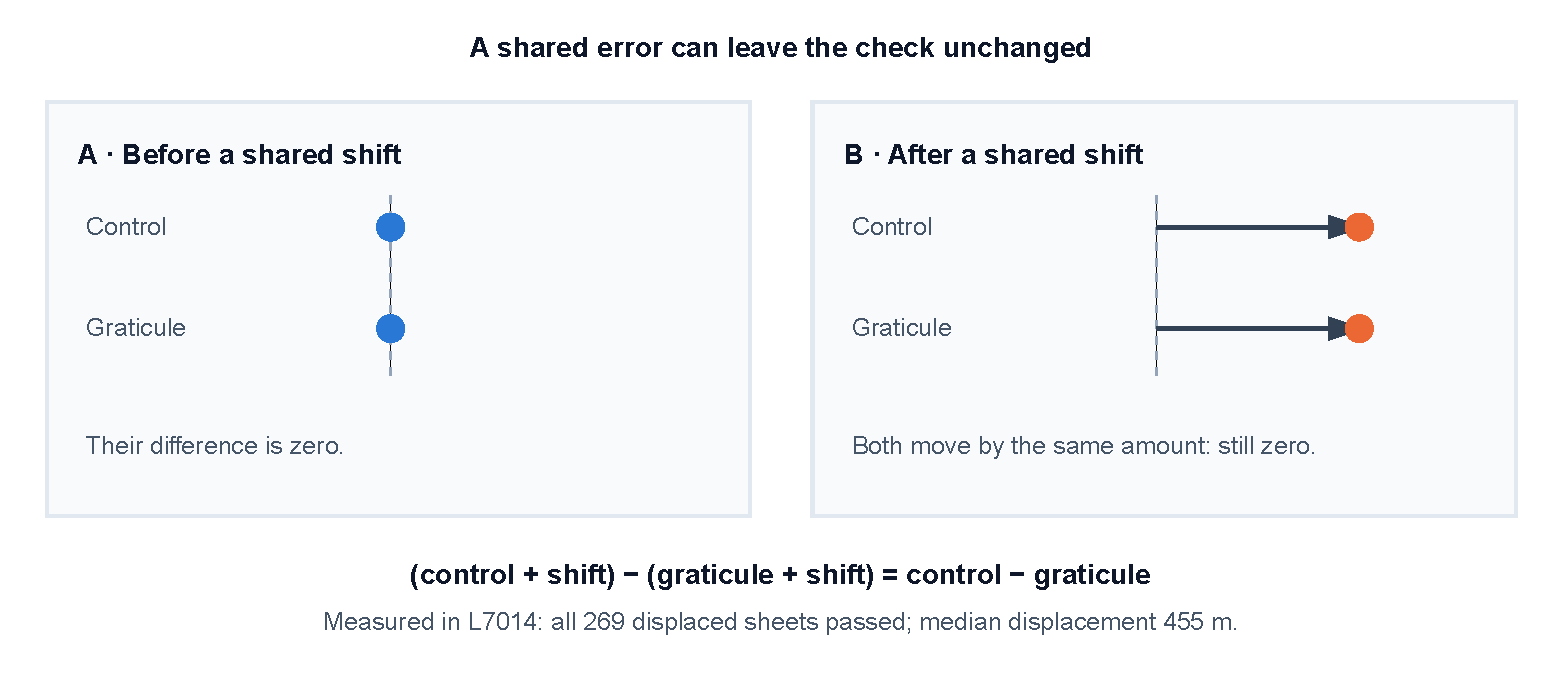
\includegraphics[width=\linewidth]{figures/figure-1.pdf}
\caption{Why a wrong position can pass an internal check. The two panels are a schematic of a shared translation, not measured sheet positions. If both operands move together, their difference stays unchanged. In the controlled L7014 reproduction, all 269 displaced sheets passed the graticule check despite a median CRS displacement of 455 m.}
\end{figure}

\bigskip\hrule\bigskip

\section{Related work}

\subsection{Georeferencing a sheet series from its own content}

The nearest prior work is Luft and Schiewe (2021), who georeference sheets of the \emph{Karte des Deutschen Reiches} 1:100,000 from their content: they segment the blue water symbols, match the resulting binary mask against OpenStreetMap water rasterised into each candidate sheet's bounding box, take the sheet with the most RANSAC-consistent patch matches, and finish with an ECC registration of content against reference. They report 96\% correct sheet identification over 56 sheets and a median georeferencing error of 101 m. What concerns us is not the matcher but the yardstick. Because a line-preserving transform spreads its error linearly, the extreme always falls at a corner, so they hold the transformed corners against "their expected positions in the series' sheet layout", and they state the consequence in print: "the alignment of corners also directly determines the ability to seamlessly join neighbouring transformed map sheets, which is a major concern for map users." Using the series' own lattice as the standard against which a sheet is judged is therefore established practice. The check we describe in §7.2 confirms it on a second series and a different frame; it does not introduce it.

Two properties of that construction bound what the yardstick can see, and both are this paper's subject. The first is that the sheet-layout bounding boxes are prior knowledge — "constructed in advance from the map series' metadata" — and are used twice: once to give the output image its spatial reference, and once as the ground truth the transformed corners are measured against. The number that results is the residual of the image registration \emph{inside an assumed frame}. Should the frame itself be wrong — the datum, not the alignment — both sides of the comparison move together and the residual does not move at all. Luft and Schiewe are explicit that the corner metric is designed to exclude one class of error: corners are used because "neatlines are the first thing constructed and have the least projection error, [so] they can be assumed to be drawn at the 'correct' place", which keeps surveying and drawing error out of the measurement. It keeps datum error out of it too. §7.4 reports a several-hundred-metre datum fault across part of the 437-sheet L7014 denominator, which a check of exactly this shape passes without a single rejection.

Luft and Schiewe say as much about a third study, and the remark is the clearest statement of this paper's thesis we have found in the prior literature. Comparing their own result with Burt, White, Allord, Then and Zhu (2019), who georeference USGS topographic sheets from neatline corners and graticule intersections, they note that those authors reach "almost perfect accuracy of 1–4 px RMSE" and immediately qualify it: the figure "reflects the detection accuracy of graticule intersections on the map image and is hardly influenced by the georeferencing process itself." That is precisely the distinction Table 1 formalises — a residual reports the relation it measures, not the one its reader wants — observed in passing rather than developed. We take it as a precedent for the argument, not as a gap.

The second is that the seam is asserted rather than measured. Corner displacement is computed per sheet against the layout and averaged over four corners into a single value; no two neighbours are ever compared to each other. A per-sheet residual cannot separate a sheet that sits slightly off its cell from two sheets that claim the same cell — the failure that caught \texttt{\detokenize{Ha Noi}}, 75 km from the city it is named for while satisfying every per-sheet check (§7.2). Inter-sheet agreement as a \emph{constraint} is well established: Janata and Cajthaml (2020) adjust a 250-sheet series under explicit adjacency conditions. We treat unforced inter-sheet agreement as a diagnostic in this archive, without claiming priority for that use.

Gede and Varga (2021) are the closest prior route to the Indochine method in §6. They detect the map-content corners, recognise a sheet identifier by OCR, derive the quadrangle from that identifier against a known layout, and use the corners as GCPs. Their geometric analysis automatically filters false corner detections. Our sheets differ at the decisive step: they print their own corners in grades from Paris and have no identifier-to-extent table, so the coordinate reading replaces the lookup. Uhl et al. (2018), in turn, use GCP displacement vectors as a per-sheet anomaly measure across map archives. Both methods reinforce the point of this paper: a useful per-sheet diagnostic is not thereby a diagnostic of a fault that belongs to the series frame.

Heitzler, Gkonos, Tsorlini and Hurni (2018) belong to the same graticule-intersection family as Burt: they locate grid intersections with a Hough transform and warp each coordinate cell independently rather than the sheet as a whole, reporting per-module precision on 20 sheets — 100\% corner detection, 94.6\% grid-intersection placement, 95.6\% coordinate interpretation — but no ground-distance error anywhere in the paper. Their only demonstration that the result improves on the existing georeferencing is a single adjacent-sheet pair: a stream's topological break across the seam closes under their method while a road's mismatch persists in both, and they note that the latter needs conflation rather than better georeferencing. One pair, chosen, unmeasured — but it is the same reflex §7.3 turns into a census: the seam is already the evidence a reader reaches for, before anyone counts it.

\subsection{Inter-sheet agreement, spent as a constraint}

Inter-sheet agreement has been used before, as a constraint. Janata and Cajthaml (2020) adjust 250 sheets of the First Military Survey of Bohemia in a single least-squares solution — 6,849 control points, more than 27 per sheet — in which the coincidence of shared sheet edges enters as a set of condition equations, robustified by iteratively reweighted least squares under Huber's M-estimate. The series was mapped \emph{à la vue} and has no geodetic basis, so no projection can be inverted and the sheet edges are the only geometry available a priori; using them is the right move, and their best solution reaches 280 m RMSE on a corpus whose own drafting is far coarser than that. The consequence for verification is structural rather than accidental. Once edge identity is imposed as a condition, "the adjacent edges fit exactly together" by construction, and the seam residual is identically zero however the mosaic as a whole is placed. Information spent as a constraint cannot be spent again as a diagnostic. The seam census we report in §7.3 is legible only because no adjacency condition was applied.

This is the same shape as the limit described in §2.1, arrived at by a different route, and neither is a defect in the work that exhibits it: Luft and Schiewe cannot see a frame error because the frame stands on both sides of their metric, and Janata and Cajthaml cannot see a seam error because the seam is an input to their solution. What the two have in common is that the quantity a reader would most naturally reach for as evidence of correctness is, in each case, the quantity the method has already committed to. We take this as the general statement of the problem rather than as a gap in the literature.

Both papers also report the limits of their own instruments, which is the register this one adopts. Janata and Cajthaml assembled about fifty control points, held out from the adjustment, to decide whether their mosaic or the Mapire.eu layer was better placed, and reported that "it is not possible to unambiguously decide which dataset is better adjusted" — the medians agree at about 250 m and fifty points do not cover Bohemia. They separately report a null on weighting control points by object category. We report comparable nulls in §8.

\subsection{Per-sheet consistency checks}

Meijers and Schoonman (2025) reach the neatline the way we do and applies a substantial per-sheet check set. MapEdge detects the frame of 557 sheets across three 1:50,000 series by taking 1D black-pixel profiles along each axis of a low-resolution overview, ranking candidate peak pairs by a fuzzy metric over separation and expected position, then repeating the profile on full-resolution edge strips cut into patches, fitting a line per side by RANSAC and intersecting the four lines. The corners serve as both the control points and the mask, at about 15 s per sheet. Both that method and ours read the same quantity off the same strips; the difference is peak selection, where MapEdge ranks candidates against a user-declared fuzzy width prior and we take an unthresholded \texttt{\detokenize{argmax}} because on these sheets the thick neatline is the darkest thing on the strip by a factor of three. Ours needs no prior and cannot be tuned; theirs adapts to layouts ours would fail on.

What matters here is the battery of five checks applied afterwards: sufficient rim samples and RANSAC inliers; an internal test that opposite sides and diagonals agree; an external test of documented sheet size in centimetres times scan dpi against the measured pixels; the distribution of inlier perpendicular distances, which detects paper bulging or caving; and a visual contact sheet of every detected corner. The battery works — on three sheets it revealed that sheet-size exceptions had been digitised wrongly in the authors' own sheet index, which was corrected as a result. These checks concern per-sheet geometry. Our §7.2 example has internally coherent readings while occupying another sheet's cell. We did not run the MapEdge implementation on that sheet; the comparison concerns the scope of internal geometric checks, not an observed MapEdge verdict.

Meijers and Schoonman also state in print the failure our own detector hits: "linear features, such as graticule lines, can occupy the same number of black pixels as the neat line." §6 reports a worked case of exactly that — a walk stopping on the graticule band, 40 px and 170 m short, every edge rejected — and what we do about it. We take this up as the open problem its author names, not as a deficiency we found.

\subsection{Verification beyond geometry}

External evidence is also used in automatic georeferencing, but it answers a different question from the internal checks above. Milleville, Verstockt and Van de Weghe (2022) geocode recognised toponyms, filter candidate locations and score predictions against independent official metadata polygons or GeoTIFF corners. Their reported mean errors are 316 m and 287 m on two adjacent-sheet corpora. Their own caution is directly relevant here: centre error can agree while the predicted extent remains wrong. An apparently simple metric is only evidence for the property it actually measures.

Text and image understanding methods extend the available evidence but do not remove that constraint. Wijegunarathna, Stock and Jones (2025) report approximately 1.03 km mean error for locality georeferencing from textual descriptions; Namgung and Chiang (2022) use spatial relationships among words to improve post-OCR rather than treating a map as a line of prose. mapKurator (Kim et al., 2023) and the ICDAR 2024 MapText competition (Li et al., 2024) demonstrate the scale at which map text can now be detected, recognised and linked. These are important routes toward independent reference, but they are not substitutes for stating what a geometric check can and cannot observe. We therefore use outside information only where it separates competing datum hypotheses (§7.5), rather than presenting it as a universal ground truth.

Recent multi-sheet work makes the same distinction from another direction. Kuna, Panecki and Zawadzki (2024) identify a difference between the mathematical framework and topographic content as a source of error accumulation during mosaicking; they caution that, despite good geometric parameters, a grid without the correct datum relationship is “not a reliable element of the mathematical framework”. They then rectify all 60 sheets of their corpus against an independently generated grid. Xu, Li and Lv (2026) likewise construct an external reference grid to supply conjugate control points for batch georeferencing. These studies do not make our blindness claim, but they show why the independence of a frame cannot be assumed from a low internal residual: it is a design choice that has to be stated. In a related operational setting, Ingensand, Lecorney and Blanc (2022) describe validation indicators based on GCP count, computed error and GCP coverage. Those indicators are useful gates; Table 1 specifies the error classes they leave outside their scope.

Tyagi and Dubey (2026) read printed map text with OCR and a multimodal model to derive a sheet's extent, which is the closest published neighbour to the printed-corner method in §6. We have not obtained the full text and therefore attribute no result to it. Legend detection is likewise outside this paper's scope: it concerns what a sheet depicts, not whether the sheet's spatial frame is independently verified.

\begin{figure}[htbp]
\centering
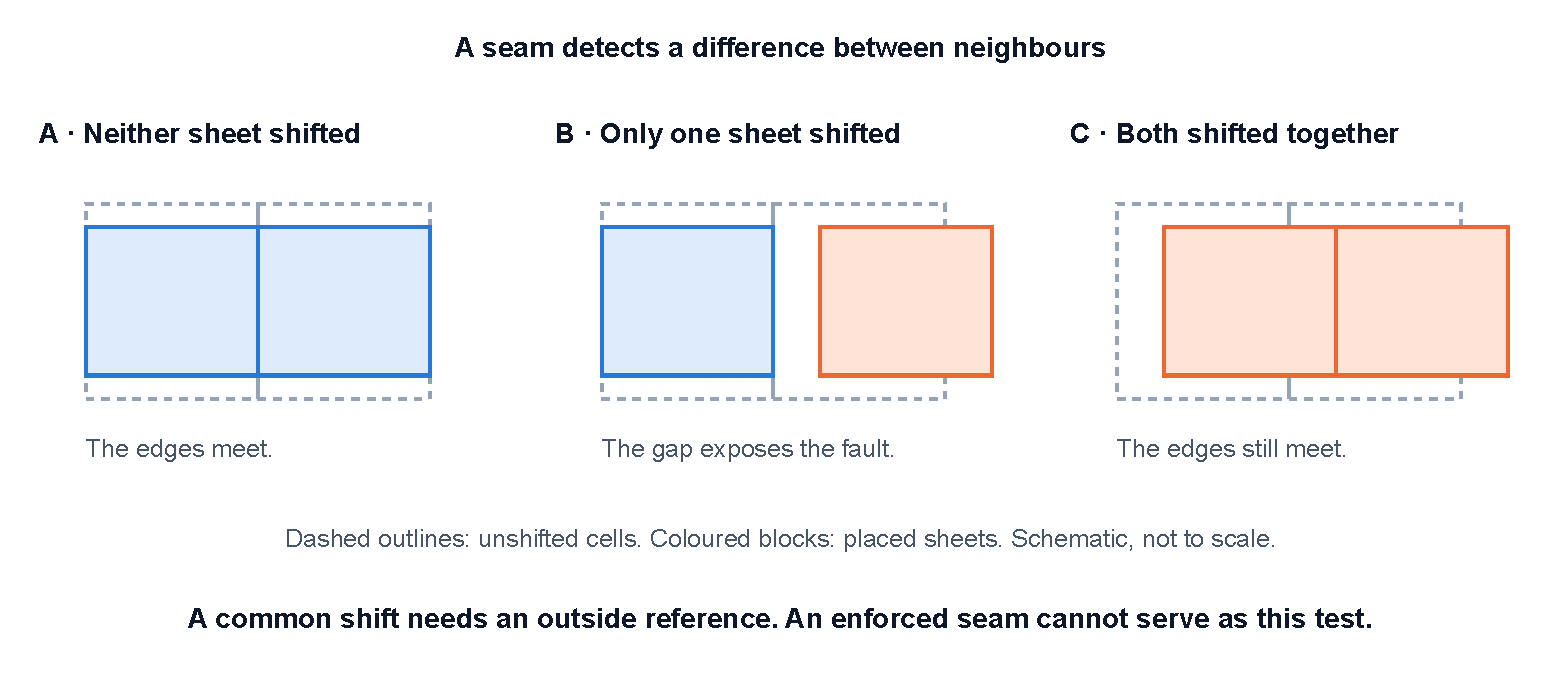
\includegraphics[width=\linewidth]{figures/figure-2.pdf}
\caption{When a seam can reveal a displacement. Schematic, not to scale. A gap opens when neighbouring sheets move differently (B); a common translation preserves their join (C). The census is diagnostic only when adjacency was left free during the warp. Figure 6 shows the geographic populations that make case B possible in this archive.}
\end{figure}

\bigskip\hrule\bigskip

\section{Corpus}

The corpus comprises a Cold-War and a colonial Vietnamese sheet series. L7014 is the US Army Map Service 1:50,000 coverage of Vietnam, held as GeoPDFs by the Perry-Castañeda Library at the University of Texas at Austin. The second is the Service géographique de l'Indochine 1:25,000 coverage of Tonkin and Thanh Hóa, held by Cartomundi at Aix-Marseille Université/CNRS. The archive previously reported a combined total of 514 sheets, comprising a 452-sheet L7014 publication count and 62 pipeline-georeferenced Indochine sheets. Because the 452 is a hand-maintained publication constant that cannot be checked against the missing serving manifest (§7.6), the sum is an archive-reported total, not a verified count of processed or currently served sheets. The measured populations below supply the denominators for the results. The L7014 material dates from the 1960s–70s; the Indochine material from 1903–1927.

Several L7014 denominators appear below and they are not interchangeable; Figure 6 shows all of them on one map; Figure 3 separates the audit populations. The series index names \textbf{627} cells. \textbf{510} of those are held as GeoPDFs. Of the 510, \textbf{448} reach the graticule check after 62 files are excluded for missing control. The check rejects 11, leaving \textbf{437} successfully warped files in the faulty build, and it is this 437 that the datum measurements in §7 are taken over. A further \textbf{24} sheets are georeferenced by hand rather than from embedded control, and sit outside that fault. The \textbf{452} in the published mosaic is a hand-maintained constant rather than a count read back from the serving manifest, and a corrected rebuild produces 436; we report it as the archive's own claim about itself and flag it in §7.6 rather than silently substituting a number the live layer cannot confirm. On the Indochine side, \textbf{79} cells are indexed and \textbf{75} held; \textbf{62} were georeferenced by the pipeline, \textbf{58} were read independently for the lattice check in §7.2, and the IIIF survey in §7.7 covers the \textbf{83} image sources those sheets resolve to, some cells holding more than one edition.

The two series are deliberately unlike in how they supply spatial evidence. L7014's source PDFs carry GCPs and a CRS declaration but require a test of that declaration. The Indochine sheets carry no embedded georeference but print corner coordinates and a regular quadrangle scheme. This contrast is useful for the paper's question: the checks in §7 do not depend on a single ingestion route, but on relations a sheet series makes available after its coordinates have been read.

The corpus is not a representative sample of all historical maps of Vietnam, nor is it a ground truth dataset for absolute positional accuracy. Its holdings, digitisation quality and availability follow the decisions of the contributing institutions. The findings below should therefore be read as a failure taxonomy demonstrated on two well-structured series, not as a benchmark ranking against methods that recover a sheet's location from no prior spatial information.

\begin{figure}[htbp]
\centering
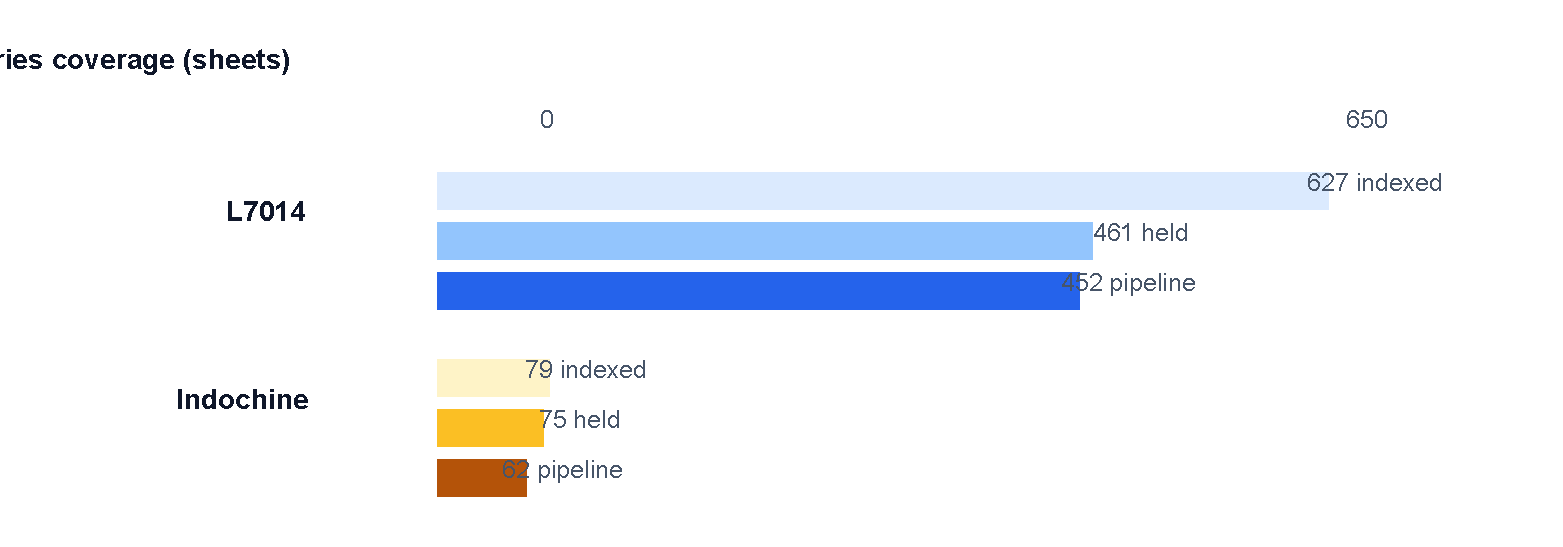
\includegraphics[width=\linewidth]{figures/figure-3.pdf}
\caption{Choose the denominator that belongs to the question. The L7014 reproduction, Indochine audits and historical processing total count different populations. “Placed” uses the CRS-displacement classification; “on cell” uses the fit check. They must not be treated as the same test. The 452-sheet publication constant is not verified against the live manifest.}
\end{figure}

\section{C1 · Modelling the survey}

The archive models three related but non-interchangeable things: a survey cell, a sheet the archive can serve, and a physical printing held by an institution. A cell is the quadrangle named by a series key and sheet number. A served sheet records the archive's present route to that cell, whether as a \texttt{\detokenize{maps}} row, a raster in a pre-tiled mosaic, or an unheld gap. A printing records an edition at a particular institution, including its title, date, part and source identifier. The distinction is not abstract: the same cell can be reprinted years apart, renamed, or issued as eastern and western halves before a later assembly.

This model makes the denominator visible. The ordinary \texttt{\detokenize{maps}} table contains only successful archive objects, so it cannot distinguish a survey of nine sheets from a survey of 627 cells of which nine have been acquired. A series index supplies that denominator. It also prevents duplicate editions from being counted as extra geographic cells, while retaining their bibliographic differences at the printing level.

Status is derived rather than stored: whether the archive holds or serves a cell follows from the current route and source records. Likewise, the printing index has no foreign key to the archive's own sheet table. An institutional printing for an as-yet unindexed cell is precisely the discovery the index exists to record; rejecting it because the archive does not already possess the cell would turn new catalogue knowledge into an import error. The same separation lets the dry run in §7.6 validate a corrected representation before the serving mosaic is changed, and it supplies the adjacency and occupancy relations required by the seam and lattice checks.

\section{C2 method A — L7014}

L7014 is a case where georeferencing control already arrives with the object. Each US Army Map Service 1:50,000 GeoPDF carries ground control points and a printed neatline. We convert the control points into a VRT, clip the image to its neatline, warp the clipped image to Web Mercator, and build the resulting rasters into one PMTiles archive. A compact companion index holds an outline, sheet number, name, edition and date for each constituent sheet. The choice of a pre-tiled archive is a serving decision: it turns a large series into one static object-store resource rather than a tile server or hundreds of per-view requests.

The procedure is intentionally conservative about what the source file establishes. Embedded GCPs locate the raster under the source's CRS claim; the neatline determines what part of the scan is map rather than collar, legend or paper. Neither fact verifies the CRS claim, and neither independently tests a join after the warp. The rest of this paper follows from taking those limits seriously. In particular, the datum fault in §7 was not a failure to find control points or to execute a warp. It was a failure to test an assumption carried by both.

Figure 4 shows what a single sheet makes available, and why those two facts are not independent evidence about each other. The sheet prints its own corner coordinates and, in its collar, the datum those coordinates are expressed in. A check that reads control points under the declared datum and compares them with the printed graticule is therefore comparing two quantities that a datum error moves together — the mechanism §7.4 measures.

\begin{figure}[htbp]
\centering
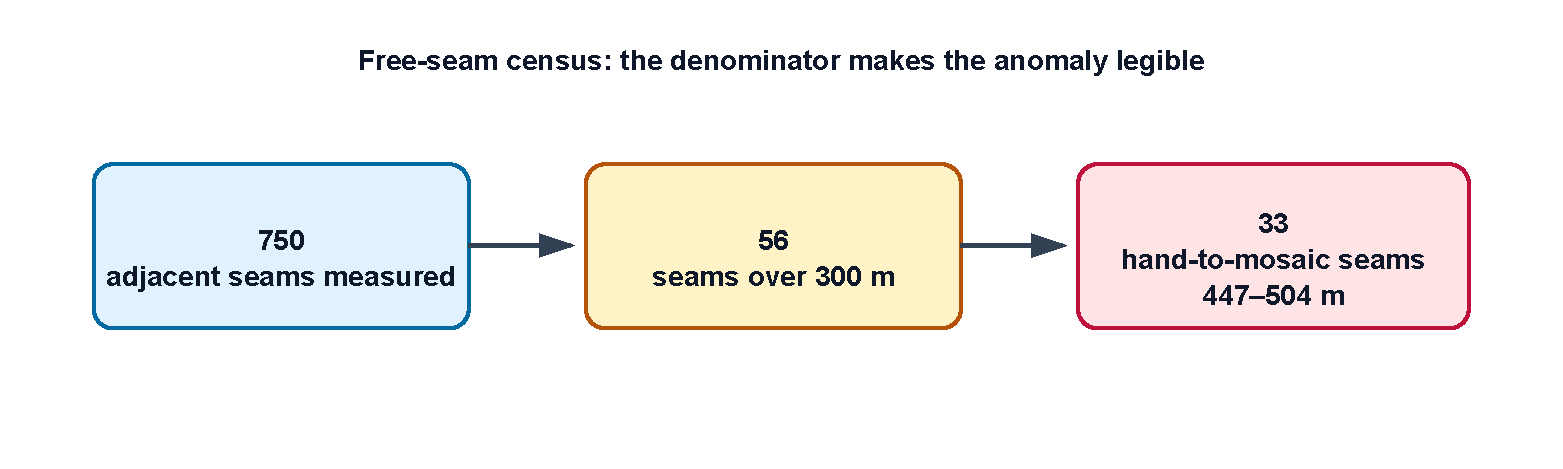
\includegraphics[width=\linewidth]{figures/figure-4.pdf}
\caption{The source of the shared assumption. The graticule and the control points are interpreted in the sheet’s declared datum. Their agreement can test internal consistency but cannot independently establish that datum. This correctly placed sheet illustrates the inputs, not an example of the measured displacement. A Lưới 6441-4, AMS Series L7014 (US Army Map Service; scan by the Perry-Castañeda Library, University of Texas at Austin). US Government work, public domain.}
\end{figure}

\section{C2 method B — Indochine}

The Indochine 1:25,000 series has no embedded georeference, but it prints the required information. On each sheet, four corner labels give longitude and latitude in grades from the Paris meridian. We detect the pixel positions of the inner neatline, OCR the four short labels just inside its corners, convert grades to degrees by multiplying by 0.9, add 2.3372 degrees for the Paris-to-Greenwich offset, and write the resulting four control points as a Georeference Annotation. On Như Trác, for example, the printed box converts to 18.75 by 12.48 km with aspect ratio 1.50, while the detected neatline measures 4,496 by 3,014 px with aspect ratio 1.49. These are independent checks on the reading, not a claim that four corners exhaust the sheet's geometric uncertainty.

The detector differs from a simple inward edge walk because the printed layout has several plausible linear features. From the paper edge inward sit a thin line, a thick neatline, another thin line, blank paper, and a graticule band. An inward walk stops at the graticule band: on Như Trác, 40 px or about 170 m short, with 14–41 px residuals and all four edges rejected. We instead fit the thick neatline. It is the darkest feature in the edge strips by a factor of three, so its per-patch choice is an unthresholded \texttt{\detokenize{argmax}}; the fitted line then supplies both the side position and the scan's rotation. The rim is only sought after de-tilting and averaging a narrow strip along that line.

Two implementation constraints follow from the scans rather than from an aesthetic preference. The rough pass averages a narrow band, not half a sheet: scans can be up to 0.8 degrees off square, and a half-sheet average smears a ten-pixel line across 30 pixels, moving Như Trác's top neatline by 35 px. And the rotation is solved once from all four sides. Independently fitted side slopes differ by only about a thousandth, but over several thousand pixels that is enough for opposite sides of a quadrilateral to differ by 14 px where the projection predicts four. One global angle preserves a single sheet geometry; each side subsequently retains only its own offset.

The method does not conceal its remaining ambiguity. The rim is a pair of thin lines seven pixels apart. We select the inner line because it gives 0.29\% disagreement between the two ground-scale estimates, rather than 0.49\% for the outer line, and because it bounds the drawn map. That preference is below the roughly 0.3\% floor set by paper shrinkage and detection noise. Reading the printed graticule ticks would resolve it and would supply interior control points; it is deferred rather than represented as an achieved precision.

\bigskip\hrule\bigskip

\section{C3 · Verification}

\subsection{What a series already knows about itself}

The lattice, the seams, the rim constant and the sheet numbering are all prior knowledge a series carries about itself, and each supports a check. The checks do not overlap the way their surface similarity suggests. \textbf{Table 1} states this paper's thesis: rows are checks, columns are error classes.

\textbf{Table 1 — which check sees which error class.} Legend: \textbf{\ensuremath{\checkmark}} can flag it under the stated inputs · \textbf{·} not established as a diagnostic here · \textbf{—} not applicable · \textbf{\ensuremath{\varnothing}} the specified fault cannot disturb the constrained or shared-input comparison · \textbf{†} only where the fault is \emph{partial} across the series, so that a displaced sheet borders an undisplaced one; a displacement common to every sheet leaves every seam closed (§7.3).

\begin{landscape}
\begin{center}
\footnotesize
\begin{longtable}{|>{\raggedright\arraybackslash}p{0.220\textheight}>{\raggedright\arraybackslash}p{0.090\textheight}>{\centering\arraybackslash}p{0.138\textheight}>{\centering\arraybackslash}p{0.138\textheight}>{\centering\arraybackslash}p{0.138\textheight}>{\centering\arraybackslash}p{0.138\textheight}>{\centering\arraybackslash}p{0.138\textheight}|}
\hline
check & scope & misregistration inside the frame & the frame/datum itself wrong & two sheets on one cell & sheet-index entry wrong & serving/tile fault \\ \hline
\endfirsthead
\hline
check & scope & misregistration inside the frame & the frame/datum itself wrong & two sheets on one cell & sheet-index entry wrong & serving/tile fault \\ \hline
\endhead
Corner residual vs sheet layout — \emph{Luft \& Schiewe 2021} & per-sheet & \ensuremath{\checkmark} & · & · & · & — \\ \hline
Internal consistency: sides, diagonals, cm×dpi, paper bulge — \emph{Meijers \& Schoonman 2025} & per-sheet & \ensuremath{\checkmark} & · & · & \ensuremath{\checkmark} & — \\ \hline
\texttt{\detokenize{graticule_error}} — sheet's GCPs vs the graticule it prints & per-sheet & \ensuremath{\checkmark} & \textbf{\ensuremath{\varnothing}} & · & · & — \\ \hline
Adjacency as a least-squares constraint — \emph{Janata \& Cajthaml 2020} & inter-sheet & \ensuremath{\checkmark} & · & · & · & — \\ \hline
…the same adjacency read back as a residual & inter-sheet & \textbf{\ensuremath{\varnothing}} & \textbf{\ensuremath{\varnothing}} & \textbf{\ensuremath{\varnothing}} & \textbf{\ensuremath{\varnothing}} & — \\ \hline
\textbf{Seam census} (adjacency left free) & inter-sheet & \ensuremath{\checkmark} & \textbf{\ensuremath{\checkmark} †} & \ensuremath{\checkmark} & · & — \\ \hline
\textbf{Lattice residual} & series & \ensuremath{\checkmark} & · & · & \ensuremath{\checkmark} & — \\ \hline
\textbf{Lattice collision} & series & · & · & \textbf{\ensuremath{\checkmark}} & \ensuremath{\checkmark} & — \\ \hline
\textbf{\texttt{\detokenize{pick_crs}}} — registration points scored against the adopted cell (§7.5) & per-sheet + index & · & \textbf{\ensuremath{\checkmark} ‡} & · & · & — \\ \hline
\textbf{Tile-key audit} & serving & — & — & — & — & \textbf{\ensuremath{\checkmark}} \\ \hline
\end{longtable}
\end{center}
\end{landscape}

\textbf{‡} Detects disagreement with the adopted frame when a cell score is available. The candidate and reference cell share Helmert parameters; the decision does not validate those parameters against independent absolute control. Table entries describe diagnostic scope, not measured detection rates from running the published methods on this corpus.

Three cells carry the argument, and each is sourced to a different paper's own design.

First, \texttt{\detokenize{graticule_error}} on "frame/datum wrong" is \ensuremath{\varnothing}, not \texttt{\detokenize{·}}. It does not merely miss the fault; it cannot report it under those shared-input conditions. The sheet's control points are read into the sheet's own datum and compared against the graticule that same sheet prints, so a datum error moves both sides together — the check passed all 269 displaced sheets, and returns 2.167e-12 on a sheet it places correctly (§7.4). Luft and Schiewe's corner metric has the same shape, and says so without meaning to when it justifies corners on the grounds that neatlines "can be assumed to be drawn at the 'correct' place".

Second, adjacency-as-constraint turns an entire row to \ensuremath{\varnothing}. Once edge identity is a condition equation, the edges fit by construction; the information was spent. Our seam row is the same measurement left unspent, and it is the row that caught the fault (§7.3).

Third, the internal per-sheet checks listed here do not establish unique occupancy. The \texttt{\detokenize{Ha Noi}} example has coherent internal readings but conflicts with another sheet's cell assignment (§7.2). This is a scope argument, not a measured result from running MapEdge on \texttt{\detokenize{Ha Noi}}. A check supplied with an independently verified sheet-to-cell assignment could detect a misplaced sheet individually; internal geometry alone cannot establish that assignment.

The claim this table licenses:

\begin{quote}\itshape
A verification instrument can remain insensitive to an error shared by its inputs or removed from its residual by an imposed constraint. Interpreting its residual therefore requires stating the comparison, the committed assumptions, and the faults capable of disturbing it.
\end{quote}

It does not claim that the lattice is novel, that adjacency is novel, or that any of these papers made a mistake. Every \ensuremath{\varnothing} is the ordinary consequence of a sound design — including ours, which is the worst row in the table: \texttt{\detokenize{graticule_error}} was shipped, trusted, and silent for the affected subset of the 437-sheet denominator.

\subsection{The lattice: residual \emph{and} collision}

We read 58 sheets independently, before asking whether their readings formed a series. Their west edges contain nine distinct values with a smallest step of 0.200 grades; their north edges contain fifteen with a 0.125-grade step. Both sets lie on those lattices with residual 0.000 at the precision of the printed corner readings. A separate pixel-space check reaches the same conclusion about the scan geometry: the rim-to-neatline offset has a median of 84.2 px, and all 58 sheets lie within 15\% of it. Sheet numbers introduce no row-order exceptions. These are relative checks. They establish that the readings make one internally coherent grid; they do not establish where that grid lies in a modern datum.

The lattice has a second operation that a residual cannot perform: it makes duplicate occupancy visible. \texttt{\detokenize{Ha Noi}} (sheet 20, 1903) is the useful counterexample. Its corners agree with one another, its ground scale agrees with its pixels to 0.78\%, its rim is at the series offset, and its content is unambiguously Hanoi. Yet its printed latitude places it 75 km south of the city, on the cell occupied by \texttt{\detokenize{Ninh Bình}}; the longitude is right and the latitude is a clean 0.75 grades out. These observations establish the limits of internal consistency, without claiming an observed pass from the MapEdge implementation described in §2.3. Nor would a small lattice residual: a sheet can sit perfectly on a cell that belongs to another sheet. The collision is the evidence. A collision is a review flag: it may represent intentional alternative editions, a printed index anomaly, or an archive/transcription error. Both editions are retained here pending a human decision about which explanation applies.

Residual and collision therefore answer different questions. The former asks whether independently read coordinates form the expected spacing; the latter asks whether the sheet index is one-to-one. Conflating them would make the \texttt{\detokenize{Ha Noi}} case disappear into an otherwise excellent grid.

\subsection{The seam census}

The census measures outline agreement rather than continuity of roads or other map content. The lattice identifies shared edges but does not constrain the PDF outlines. For each edge, \texttt{\detokenize{l7014_seams.py}} samples 25 equally spaced positions between 10\% and 90\% of its length, avoiding corner junctions. At each position it finds the nearest point on each outline and measures their separation using a local longitude/latitude-to-metre approximation. The edge statistic is the median of these distances; the reported census median is the median across edges. The 100 m and 300 m cutoffs summarize the observed tail, rather than define independently calibrated acceptance thresholds. For nearly straight parallel edges the distance principally reflects normal separation; it need not recover along-edge displacement or a full displacement vector.

The lattice compares sheets to the series frame. A seam compares each sheet to its neighbour while leaving that relation out of the warp. In the mosaic-only reproduction, 717 PDF/PDF seams have a median displacement of 9.2 m and 97 exceed 300 m. Splicing in the separate hand-sheet rows produces a second, hand-extended cohort of 778 seams: 36 additional JPG/PDF seams and 25 JPG/JPG seams. The hand-extended cohort has the same 9.2 m median and 111 seams over 300 m. The hand-extended cohort includes the mosaic-only cohort; the two denominators are reported separately rather than treated as independent samples.

The distribution is not a diffuse consequence of paper distortion. The 36 hand-to-mosaic seams span 1.8–446.2 m; none falls in the earlier 447–504 m band. A seam reports only the component normal to the shared edge: the hand comparisons have medians of 438.0 m east/west and 133.7 m north/south, recombining to 457.9 m, close to the 454.9 m median CRS displacement.

The hand-sheet comparisons must be distinguished from the free PDF/PDF comparisons. The hand workflow supplies lattice-derived ground corners, and the hand manifest is assembled from those ground coordinates rather than independently measured warped image boundaries. A JPG/PDF join therefore compares a PDF outline with a lattice-derived boundary. A JPG/JPG join compares two such boundaries. The 25 JPG/JPG distances of 0.0–0.6 m describe consistency of those ground coordinates, not an independent validation of either image registration. Only the PDF/PDF cohort is used as free-seam evidence here.

The two builds differ in the CRS-selection flag and in which files survive the checks. The faulty build contains 717 PDF/PDF seams, of which 189 exceed 100 m and 97 exceed 300 m. The corrected build contains 715, none above 100 m (Figure 5). To separate change in geometry from change in membership, we matched edges by their unordered sheet-ID pair. All 715 corrected edges occur in the faulty census. On these same edges, 189 fall from above 100 m to at most 100 m, with no crossings in the opposite direction; the maximum corrected edge median is 72.4 m. The two faulty-only edges measure 3.6 m and 15.6 m, so their exclusion cannot explain disappearance of the large-displacement tail. Matched-cohort medians are 9.2 m before and 6.8 m after correction.

These are descriptive comparisons within one series. Edges share sheets and are not independent replicates; their distances do not measure absolute accuracy or content alignment. The matched analysis, input hashes and excluded pairs are reproducible with \texttt{\detokenize{scripts/paper-seam-pairs.mjs}}.

This is also the limit of the instrument. What the seam census detects is \emph{differential} disagreement across a shared edge, and it fired here only because the fault was partial: a displaced sheet was somewhere adjacent to an undisplaced one. Had every sheet in the series moved by the same vector, every seam would have closed exactly as before and this census would have reported nothing. The instrument found the fault because the fault had a boundary — the boundary Figure 6 maps.

The seam anomaly was the first inexpensive indication, in this archive, that it had split into two spatial populations. The measurement needs neither a reference map nor a new set of control points: it needs only two sheets that claim to share an edge. Its value is diagnostic: it catches a disagreement that a per-sheet metric cannot see, provided adjacency has not already been imposed as a condition of the solution. A common displacement preserves a seam, just as it preserves any other relative measurement.

\begin{figure}[htbp]
\centering
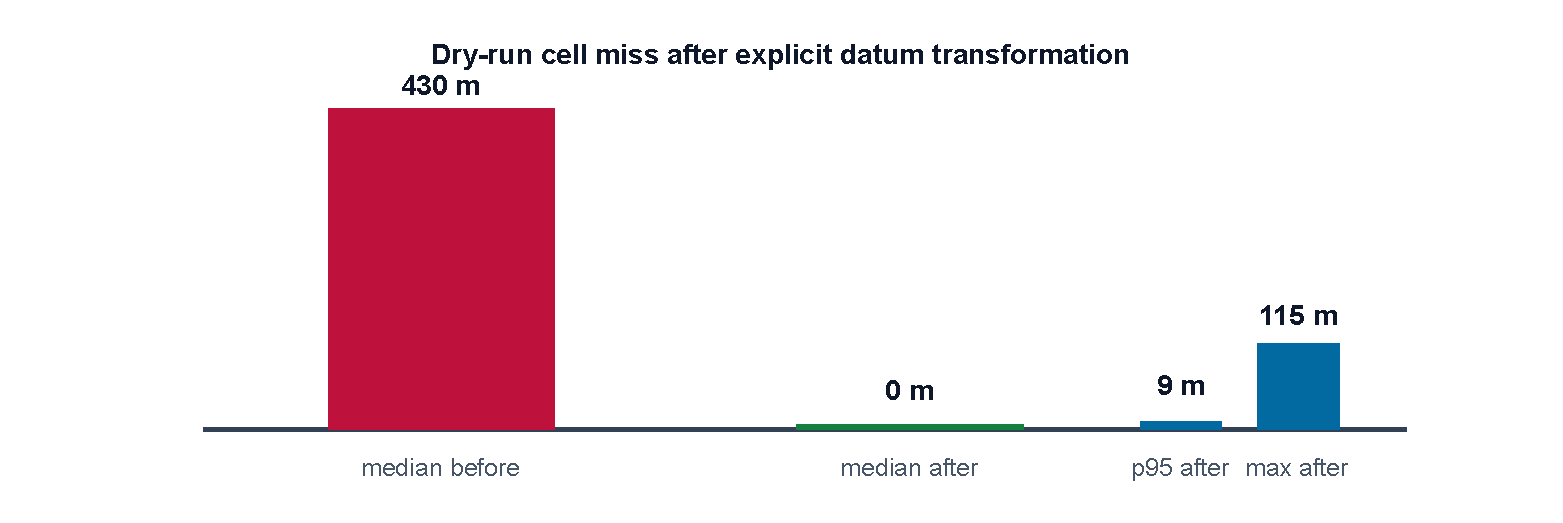
\includegraphics[width=\linewidth]{figures/figure-5.pdf}
\caption{The large-displacement tail is absent after correction. Counts of free PDF/PDF seams in each displacement bin. The faulty build has 189 of 717 seams over 100 m; the corrected build has 0 of 715. These are separate builds, not a paired analysis of the same 717 seams. A matched analysis of the 715 common edges also gives 189 versus zero above 100 m (§7.3). A small median (9.2 m before, 6.8 m after) alone would obscure the faulty build’s large tail.}
\end{figure}

A single seam has been offered as this kind of evidence before (§2.1): Heitzler et al. (2018) show one adjacent-sheet pair closing under their method, by eye, with no threshold and no denominator. What changes here is the count — 717 free seams, binned and thresholded, not one pair chosen to illustrate.

\subsection{The blind self-check}

The seam anomaly led to a datum fault in the L7014 GeoPDF pipeline. The 437-sheet denominator contains a fault population that depends on the measurement: 276 sheets under the fit criterion and 269 under the CRS-displacement criterion. Their displacements span 395–528 m, with a median of 455 m. Some files carried an NGA LGIDict datum label that GDAL could not map and were warped after a warning with a WGS 84 fallback. More subtly, even a sheet explicitly labelled \texttt{\detokenize{Indian_1960}} could fail: the \texttt{\detokenize{EPSG:4131}} to \texttt{\detokenize{EPSG:4326}} operation returns the input unchanged outside its area of use. The behaviour is non-uniform: a probe at 106.00 E, 16.00 N moves about 470 m, while one at 109.25 E, 13.25 N moves 0. The production archive therefore contains a discontinuity rather than one uniform translation.

Our existing \texttt{\detokenize{graticule_error}} check did not report it. In the faulty pass, 448 files reached the check after 62 were excluded for missing control. It rejected 11 and retained 437, including all 269 with reproduced CRS displacements of 395–528 m. This is not a sensitivity limit: the rejections it did issue fire between 0.004 and 0.076 degrees off the printed graticule, so the instrument has a working dynamic range and still returned nothing on a 455 m translation. On A Lưới — which \texttt{\detokenize{pick_crs}} resolves to its declared CRS, and whose CRS displacement is 0.0 m — it returns \texttt{\detokenize{2.167e-12}}. The implementation converts registration coordinates into the candidate CRS's own geographic coordinate system (\texttt{\detokenize{CloneGeogCS}}) and compares their extrema with the sheet's graticule metadata, or with quarter-degree snapping when those metadata are absent. That calculation does not independently test the subsequent transformation to WGS 84. It can reject inconsistent registration while remaining insensitive to the omitted datum transformation at issue here. The \ensuremath{\varnothing} in Table 1 denotes this fault's inability to disturb the comparison; it does not mean the check must return zero when other errors are present.

The same check failed a second time, in the opposite direction, and the second failure is worth recording because it is the first one's mirror. \texttt{\detokenize{graticule_error}} read its transformed coordinate pair positionally, and the two spatial-reference objects it compares disagree about axis order while reporting the same axis strategy. Every sheet the datum correction moved was therefore transposed, producing an apparent error of tens of degrees, and \textbf{370 of 437 sheets were rejected — the datum fix thrown out by the check it was meant to supersede}. Pinning both operands to traditional order took the rejections from 370 to 1. A check that cannot see a real fault and a check that rejects a real correction are the same defect seen from two sides: in neither case was the quantity being compared the quantity the reader assumed.

The fault is also not uniform across the series, and its shape is geographic rather than random. Figure 6 places all 627 indexed cells and colours each by the route its sheet took. The 269 displaced sheets fall in two groups, north and south, separated by a band between roughly 14°N and 17°N in which no sheet took the faulty route at all. That band is why a single probe can mislead: the archive holds two spatial populations, not one translated whole.

\begin{figure}[htbp]
\centering
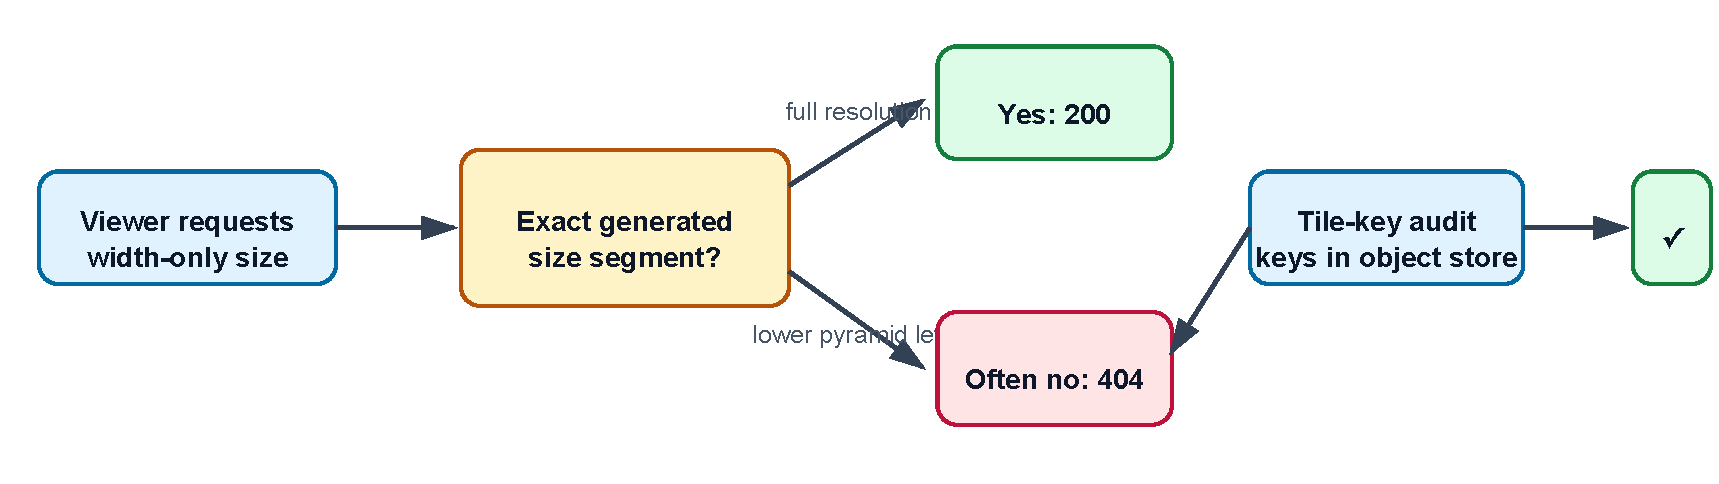
\includegraphics[width=\linewidth]{figures/figure-6.pdf}
\caption{The fault has a geographic boundary. Each square is one indexed L7014 cell. Orange marks 269 displaced sheets; blue marks 168 placed sheets. No sheet between 14°N and 17°N took the faulty route. A seam can expose the fault where these populations meet; neighbouring sheets that share a displacement can still agree. Grey and empty cells distinguish missing warp results from missing holdings. Counts describe the controlled reproduction; 452 is the archive’s hand-maintained publication claim.}
\end{figure}

\subsection{CRS selection against an adopted frame}

The corrected route adds \texttt{\detokenize{pick_crs}} before the graticule check. It scores the declared or fallback CRS and, where available, an Indian 1960 alternative with explicit Everest 1830 (1937 Adjustment) Helmert parameters. For each candidate, it transforms the registration coordinates to WGS 84 and averages, over the expected cell corners, the distance to the nearest transformed registration point. Registration coordinates come from embedded GCPs, with neatline vertices as the fallback. It selects the candidate with the smaller score only if that score is at most 150 m. If every available candidate exceeds that threshold, it rejects the sheet. If no score can be computed, however, the implementation retains the declared or fallback CRS; this case is not verified by the lattice decision.

The reference is external to an individual GeoPDF declaration, but it is not independent of the adopted datum transformation. \texttt{\detokenize{cell_corners}} transforms the index coordinates with the same explicit Helmert parameters used by the alternative candidate. Agreement therefore tests consistency with the adopted frame and can expose a missing transformation, while a shared error in those parameters could remain undetected. The result does not establish absolute accuracy at the approximately 15 m scale of the reported index-to-outline agreement. Testing that claim would require appropriately distributed reference positions whose coordinates were not generated by the same transformation.

This distinction preserves the useful result without giving the selection rule a broader authority than its inputs support. Refusal catches cases outside the scored alternatives; agreement identifies a compatible interpretation conditional on the adopted frame.

\subsection{The fix, validated without being applied}

Applying the explicit Helmert transformation in a dry run changes which sheets reach their cell at all. The corrected pass warps 436 sheets to the faulty pass's 437, and 434 of them land on their cell against 161 before. Sheets more than 150 m off their cell fall from 276 of 437 to 2 of 436. The median miss among on-cell sheets barely moves — 11 m before, 10 m after — because the correction does not improve sheets that were already placed; it moves displaced sheets onto their cells. For the same reason the worst on-cell miss rises, from 50 m to 95 m, with a net increase of 273 on-cell sheets across the two builds. The two the correction leaves off cell are \texttt{\detokenize{6630-4}} Xa Phan Thiet (mean 662 m) and \texttt{\detokenize{6349-4}} Cua Tra Ly (mean 396 m); in both the worst corner far exceeds the mean, which reads as a distorted or mis-clipped outline rather than a datum problem. The same method leaves the 24 hand-georeferenced sheets outside the fault: their control-point residuals remain 2.3–19.0 m RMS. These figures validate the proposed interpretation and correction; they do not describe a rebuilt public mosaic.

That distinction is deliberate, and the live state is worse than "uncorrected". At the time of writing the \texttt{\detokenize{l7014-20260913}} archive has not been re-warped or re-uploaded, and its sheet manifest returns 404: the build shipped pixels without the accompanying \texttt{\detokenize{.geojson}}, so \texttt{\detokenize{fit}} cannot be run against the serving layer at all and the 452 constant quoted in §3 cannot be checked against it. What readers currently receive is therefore not merely displaced but unmeasurable from outside — itself an instance of §7.7's point that a serving layer needs its own instrument. The published fault is therefore part of the result, not a historical problem retrospectively erased from the evidence. A rebuild is an operational next step; reporting the dry run separately prevents it from being mistaken for a measurement of the current serving layer.

\begin{figure}[htbp]
\centering
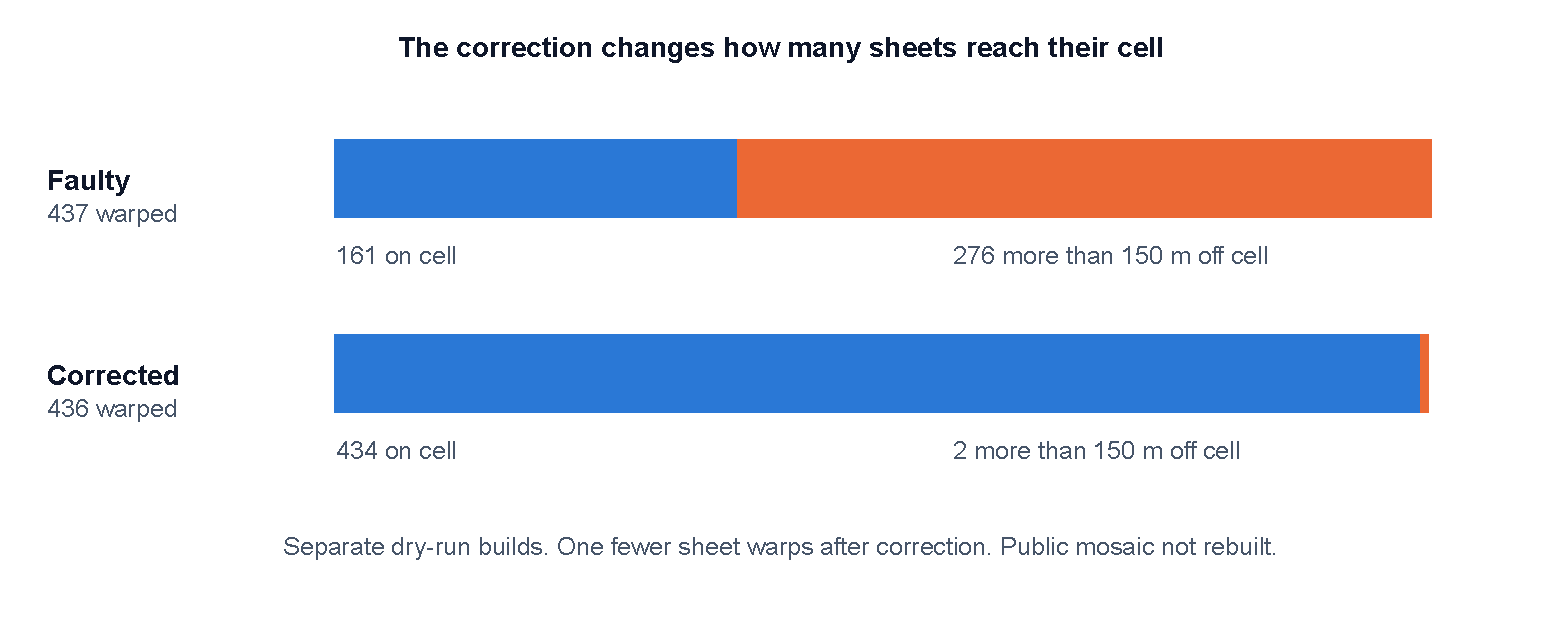
\includegraphics[width=\linewidth]{figures/figure-7.pdf}
\caption{The correction recovers cell placement in the local reproduction. Bars use a common sheet-count scale. The faulty build places 161 of 437 sheets on cell; the corrected build places 434 of 436. Orange marks sheets more than 150 m off cell. The two remaining failures require review. These results do not measure a rebuilt public mosaic.}
\end{figure}

\subsection{One layer down: a serving check}

The same scope rule applies after georeferencing, when a correct source image is requested from an image service. An audit of the Indochine IIIF endpoint found that its generated tiles use explicit \texttt{\detokenize{w,h}} size segments, whereas canonical IIIF clients, including the rendering stack used here, request a width-only segment. The two forms agree at full resolution, so a superficial whole-image test passes. One level below the overview they disagree for 58.6\% of tiles across the 83-sheet survey. The resulting 404 reads as “Source not found”, which describes neither the source nor the real fault: the endpoint cannot compute an arbitrary requested size at that scale.

This is not a georeferencing error and should not inflate the positional claims above. It belongs in the taxonomy because it demonstrates the same operational lesson at the serving layer. A successful full-resolution request does not test the tile keys a viewer will actually request. The appropriate instrument is a tile-key audit against keys present in the object store; it has no opinion about datum, lattice or seam geometry, and those checks have no opinion about it.

\begin{figure}[htbp]
\centering
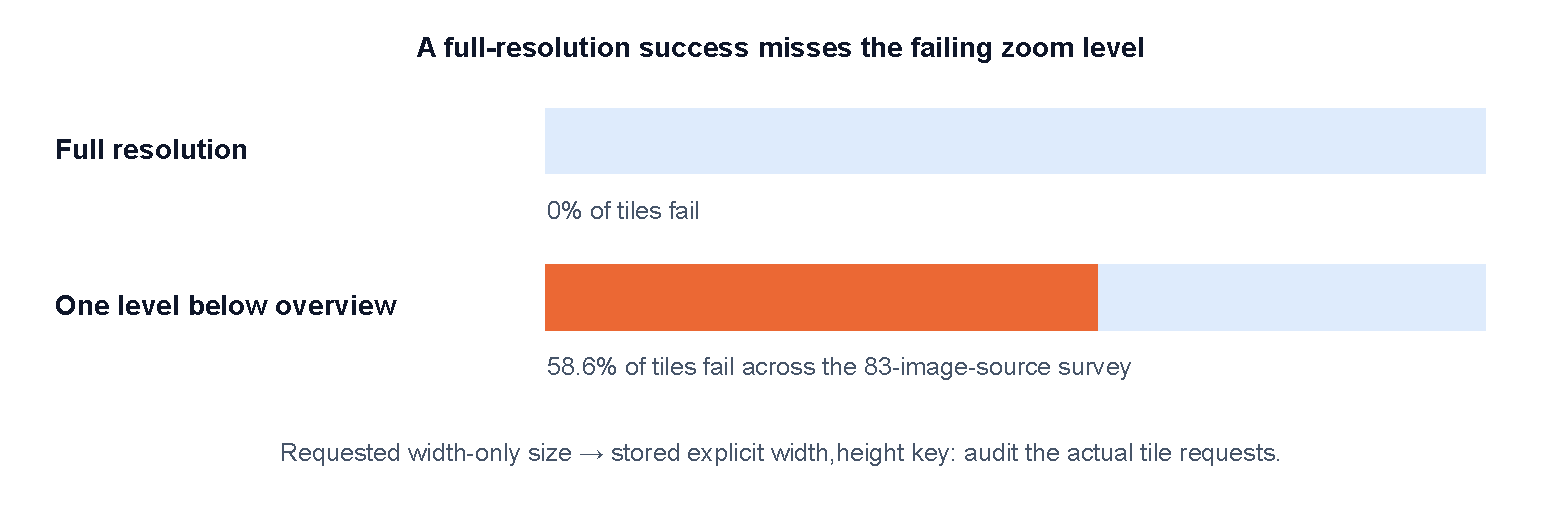
\includegraphics[width=\linewidth]{figures/figure-8.pdf}
\caption{Test the resolution that the viewer requests. Orange is the share of tile requests that fail at the stated level. Full-resolution success coexists with 58.6\% failures one level below the overview in the 83-image-source survey. This measures serving behaviour, not positional accuracy; no intermediate zoom-level rates are inferred.}
\end{figure}

\bigskip\hrule\bigskip

\section{Negative results}

Several plausible checks did not yield evidence strong enough to carry the argument. For the Indochine datum, we warped one 1903 sheet from its detected corners and compared the Red River with modern imagery. Across 794 rows the modern channel lay at a median of 58 m east of the historical one, with a ±180 m spread. That is compatible with a small east–west displacement, but the channel runs north–south and therefore provides no north–south constraint; a two-dimensional correlation peaked at the edge of its search window. River migration, not the georeference, dominates the remaining variation. The southeast confluence agrees to about 100 m, which is reassurance rather than a measurement.

Toponym lookup was less useful still. Of twenty village names transcribed from the sheet, only four returned a single OpenStreetMap result, and even an apparently good administrative match can describe a modern settlement rather than its historical core. Correlating historical ink density with modern red-roof pixels produced a smooth, peakless surface driven by the rectangular overlap of the masks. Neither result is retained as a weak positive. Both delimit what an external check would need before it could adjudicate the Indochine datum.

The image-derived method also has known exceptions. Gia Bình, Phúc Nhạc, Quất Lâm and Thái Bình need hand-placed corners because thin-frame editions or inconsistent rim offsets defeat the thick-line assumption. The unresolved pair of rim lines is worth roughly 30 m, and only the printed graticule ticks can settle it. These limitations are not failures of the lattice or seam instruments; they are limits on the quality of the per-sheet readings those instruments are asked to compare.

\section{Discussion}

The contribution is not a new universal accuracy statistic. It is a way to decide what a statistic can mean before reporting it. Every verification check has a scope, and some checks reuse a datum, frame or adjacency relation that the georeferencing procedure already assumed. Such a check may be entirely appropriate for detecting local misregistration while being incapable of detecting a shared displacement. The useful question is therefore not whether a residual is small in isolation, but which error classes could have made it small.

For a regular series, this yields a practical ordering of checks. Begin with low-cost relations the series itself supplies: lattice spacing, one-to-one cell occupancy and free seams. Use reference positions independent of the adopted transformation when absolute placement is the claim to be tested. The \texttt{\detokenize{pick_crs}} decision provides a narrower consistency check (§7.5). Do not turn a diagnostic relation into a hard constraint if it will later be the only available test of that relation. And preserve refusal as an outcome: an anomalous sheet is information for review, not an invitation to publish the least implausible transformation.

The reasoning may apply beyond these two series where its structural conditions hold. A seam census requires enough adjacent sheets, a lattice requires a known regular scheme, and neither substitutes for an independent absolute reference. Conversely, an individual sheet can receive only per-sheet checks, which is precisely why its residual must not be made to imply more. The archive model in §4 is part of the method here: series membership, editions, gaps and serving routes are not merely catalogue metadata when they determine which verification relations can be computed.

\section{Conclusion}

A georeferenced map series arrives with more evidence about itself than a single sheet can offer, and the practical question is not how much of it to gather but what each piece is still free to say. A controlled reproduction of the archive's faulty route retained 437 sheets, including 269 with CRS displacements of 395–528 m that passed the graticule check. That check cannot independently validate the transformation from the sheet's geographic CRS to WGS 84. On the same 715 PDF/PDF edges, correction reduced the number above 100 m from 189 to zero. The comparison establishes improved outline agreement. CRS selection against the lattice supplies a separate test of consistency with the adopted Helmert transformation, whose absolute accuracy remains to be independently assessed. These build measurements do not establish the exact population or accuracy of the serving archive.

The generalisable part is not the magnitude, which is particular to this archive, nor the instruments, which are not new. It is the bookkeeping: a verification check has a scope and a set of inputs it has already committed to, and those two facts determine which error classes it can still report. Table 1 is that bookkeeping for the checks we use and for three published ones, and every \ensuremath{\varnothing} in it is the ordinary consequence of a sound design — including our own, which is the worst row in the table. Stating a residual without stating its scope is therefore not a small omission. It is the omission that let a 455 m error render, pass its check, and ship.

\section{Data and code availability}

The archive's derived data — georeference annotations, sheet and printing indexes, verification outputs and code used to produce them — will be deposited under CC-BY-4.0 in a versioned Zenodo release before submission. The release DOI is intentionally not fabricated in this draft and will be inserted only after the archive record is minted. Source scans are not redistributed: they remain under their holding institutions' terms and are cited by their IIIF resources or catalogue records. This separation preserves a reproducible account of the derived geometry without asserting rights over the underlying scans.

The implementation includes the L7014 mosaic pipeline, the Indochine frame and corner-reading pipeline, the series-index migrations, and the checks described in §7. The figures ledger records the source and measurement date of every number quoted in this paper. The serving archive is also versioned separately from a proposed correction: reproducibility requires readers to distinguish the evidence measured on the current layer from the dry run that supports its rebuild.

\begin{figure}[htbp]
\centering
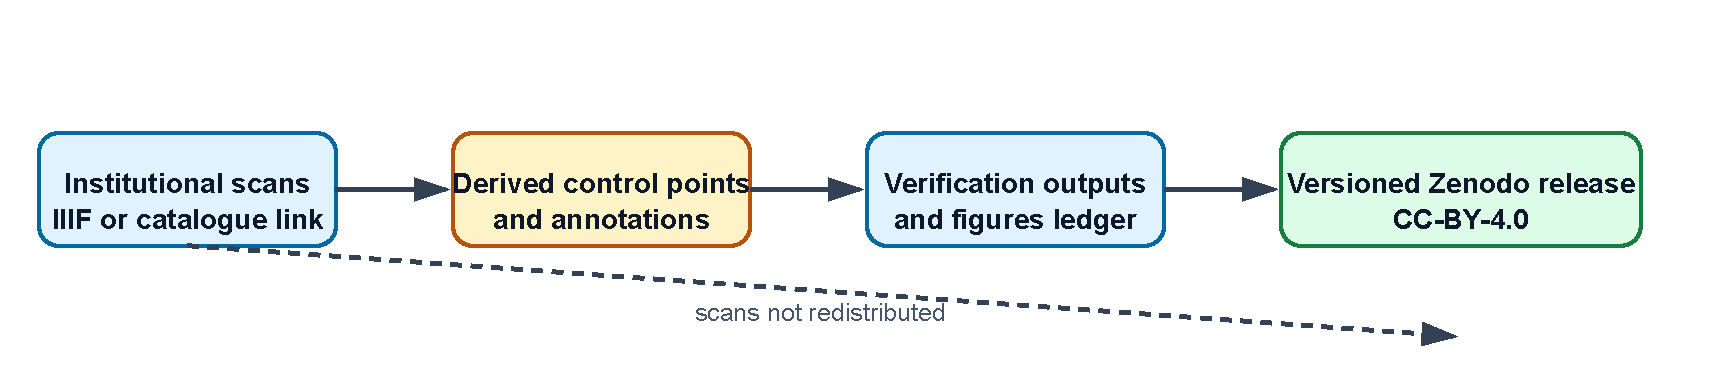
\includegraphics[width=\linewidth]{figures/figure-9.pdf}
\caption{Three states of the evidence at the recorded audit. The served archive, local experiment and planned deposit have different evidentiary roles. Only the local reproduction supports the before/after counts. A future deposit must identify its build and preserve those distinctions; a DOI has not yet been minted.}
\end{figure}

\bigskip\hrule\bigskip

\section{References}

The bibliography below contains only works cited in this draft. Every entry with a DOI was resolved against stored publisher metadata on 2026-09-20 and screened for editorial notices; none carries a retraction, correction or expression of concern. Two entries carry a year that differs from the one their publisher's house style prints, because we use the date in the publisher's own Crossref deposit rather than the volume year: Janata and Cajthaml is deposited as 30 December 2020 although \emph{Applied Sciences} 11(1) is a 2021 volume, and Burt et al. is deposited as 2019 although \emph{CaGIS} 47(1) is a 2020 issue.

\begin{itemize}
\item Burt, J. E., White, J., Allord, G. J., Then, K. M., \& Zhu, A.-X. (2019). Automated and semi-automated map georeferencing. \emph{Cartography and Geographic Information Science}, 47(1), 46–66. \url{https://doi.org/10.1080/15230406.2019.1604161}
\item Gede, M., \& Varga, L. (2021). Automatic georeferencing of topographic map sheets using OpenCV and Tesseract. \emph{Proceedings of the International Cartographic Association}, 4, 38. \url{https://doi.org/10.5194/ica-proc-4-38-2021}
\item Heitzler, M., Gkonos, C., Tsorlini, A., \& Hurni, L. (2018). A modular process to improve the georeferencing of the Siegfried map. \emph{e-Perimetron}, 13(2), 85–100. \url{http://www.e-perimetron.org/Vol_13_2/Heitzler_et_al.pdf}
\item Ingensand, J., Lecorney, S., \& Blanc, N. (2022). An open API for 3D-georeferenced historical pictures. \emph{The International Archives of the Photogrammetry, Remote Sensing and Spatial Information Sciences}, XLVIII-4/W1-2022, 217–222. \url{https://doi.org/10.5194/isprs-archives-xlviii-4-w1-2022-217-2022}
\item Janata, T., \& Cajthaml, J. (2020). Georeferencing of multi-sheet maps based on least squares with constraints—First Military Mapping Survey maps in the area of Czechia. \emph{Applied Sciences}, 11(1), 299. \url{https://doi.org/10.3390/app11010299}
\item Kim, J., Li, Z., Lin, Y., Namgung, M., Jang, L., \& Chiang, Y.-Y. (2023). The mapKurator system: A complete pipeline for extracting and linking text from historical maps. \emph{ACM SIGSPATIAL 2023}. \url{https://doi.org/10.1145/3589132.3625579}
\item Kuna, J., Panecki, T., \& Zawadzki, M. (2024). Methodology of mosaicking and georeferencing for multi-sheet early maps with irregular cuts using the example of the Topographic Chart of the Kingdom of Poland. \emph{ISPRS International Journal of Geo-Information}, 13(7), 249. \url{https://doi.org/10.3390/ijgi13070249}
\item Li, Z., Lin, Y., Chiang, Y.-Y., Weinman, J., Tual, S., Chazalon, J., Perret, J., Duménieu, B., \& Abadie, N. (2024). ICDAR 2024 competition on historical map text detection, recognition, and linking. In \emph{Document Analysis and Recognition — ICDAR 2024} (pp. 363–380). \url{https://doi.org/10.1007/978-3-031-70552-6_22}
\item Luft, J., \& Schiewe, J. (2021). Automatic content-based georeferencing of historical topographic maps. \emph{Transactions in GIS}, 25(6), 2888–2906. \url{https://doi.org/10.1111/tgis.12794}
\item Meijers, M., \& Schoonman, J. (2025). Mapping the edge: A novel approach to georeferencing historical map series. \emph{e-Perimetron}, 20(1), 12–24. \url{http://www.e-perimetron.org/Vol_20_1/Meijers_et_al.pdf}
\item Milleville, S., Verstockt, S., \& Van de Weghe, N. (2022). Automatic georeferencing of topographic raster maps. \emph{ISPRS International Journal of Geo-Information}, 11(7), 387. \url{https://doi.org/10.3390/ijgi11070387}
\item Namgung, M., \& Chiang, Y.-Y. (2022). Incorporating spatial context for post-OCR in map images. \emph{GeoAI ’22}. \url{https://doi.org/10.1145/3557918.3565864}
\item Tyagi, P., \& Dubey, V. (2026). Automated georeferencing of topographic maps via OCR and in-context multimodal LLM reasoning. In \emph{NCVPRIPG 2025 proceedings} (pp. 99–113). \url{https://doi.org/10.1007/978-3-032-08511-5_8}
\item Uhl, J., Leyk, S., \& Chiang, Y.-Y. (2018). Map archive mining: Visual-analytical approaches to explore large historical map collections. \emph{ISPRS International Journal of Geo-Information}, 7(4), 148. \url{https://doi.org/10.3390/ijgi7040148}
\item Wijegunarathna, R., Stock, K., \& Jones, C. (2025). Large multi-modal model cartographic map comprehension for textual locality georeferencing. \emph{GIScience 2025}. \url{https://doi.org/10.4230/LIPIcs.GIScience.2025.12}
\item Xu, M., Li, Q., \& Lv, R. (2026). Grid-based batch georeferencing of historical urban maps: A framework addressing control point scarcity through cartographic grouping. \emph{Open Geosciences}, 18(1). \url{https://doi.org/10.1515/geo-2025-0919}
\end{itemize}

\end{document}
